\chapter{Design of MPI\_T support in TAU}
This chapter includes co-authored material previously published in EuroMPI~\cite{EuroMPI} and Parallel Computing~\cite{ParCo}. These papers were the result of a collaboration with Aur\`{e}le Mah\'{e}o, Sameer Shende, Allen Malony, Hari Subramoni, Amit Ruhela, and Dhabaleswar (DK) Panda. I implemented the plugin support in TAU and integrated BEACON and TAU. Hari Subramoni is the lead developer of the MVAPICH2 project and Sameer Shende leads the TAU project. Aur\`{e}le Mah\'{e}o implemented the GUI support in PYCOOLR for performance monitoring. Sameer Shende designed and implemented the initial version of the MPI\_T based performance introspection in TAU and provided critical guidance in designing the plugin support in TAU. I designed and implemented the experiments described in this chapter. For the autotuning experiments on AmberMD and 3DStencil, I received support from Hari Subramoni and Amit Ruhela. 
\par The existence of MPI\_T provides an opportunity to link together the components above. However, each component must be extended to interact through the MPI\_T interface, as well as in concert with each other. Although applicable to any standard-compliant MPI implementation, the design of the MPI\_T support in TAU was performed in close collaboration with the MVAPICH2 MPI library. Below, we describe the design approach for MVAPICH2 and TAU integration to enable runtime introspection, performance tuning, and recommendation generation. Figure \ref{fig:mpitinfrastructure} depicts the infrastructure architecture and component interactions. We then present sample usage scenarios for this infrastructure. 
\section {Enhancing MPI\_T Support in MVAPICH2}
MVAPICH2 exports a wide range of performance and control variables through the MPI\_T interface. A performance variable represents an internal metric or counter, and setting a control variable may alter the behavior of the library. Current support for MPI\_T variables in MVAPICH2 broadly fall under the following categories:
\subsection {Monitoring and Modifying Collective Algorithms} 
For collective operations such as \verb+MPI_Bcast+ and \verb+MPI_Allreduce+, there are a variety of algorithms available and the right algorithm to use depends on a number of parameters such as system metrics (bandwidth, latency), the number of processes communicating and the message size. MVAPICH2 exports CVARs that can be used to determine the collective algorithm based on the message size. It also supports PVARs that monitor the number of times a certain collective algorithm is invoked.
\begin{center}
	\begin{figure*}[tbp!]
         \centering
		%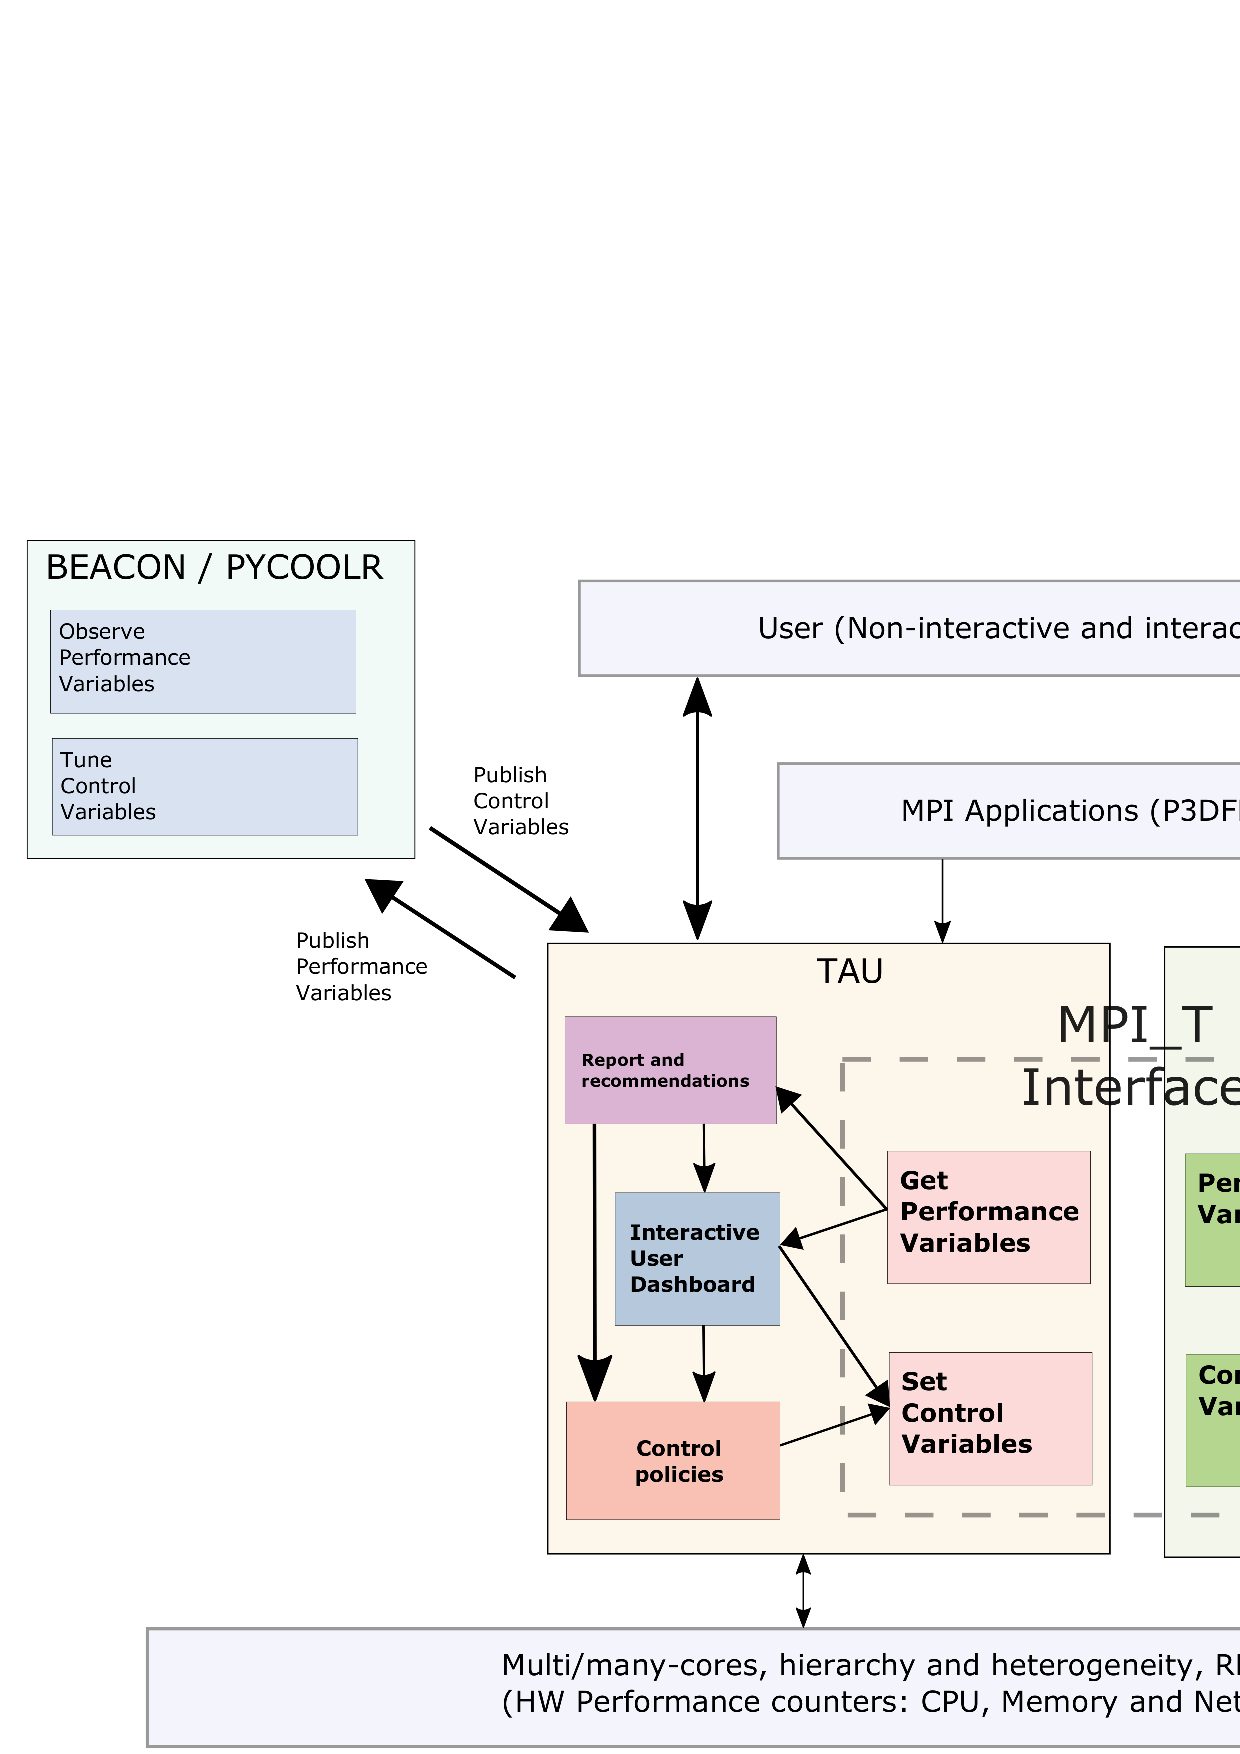
\includegraphics[width=\textwidth,scale=0.05]{figures/MPI_T_infrastructure}
		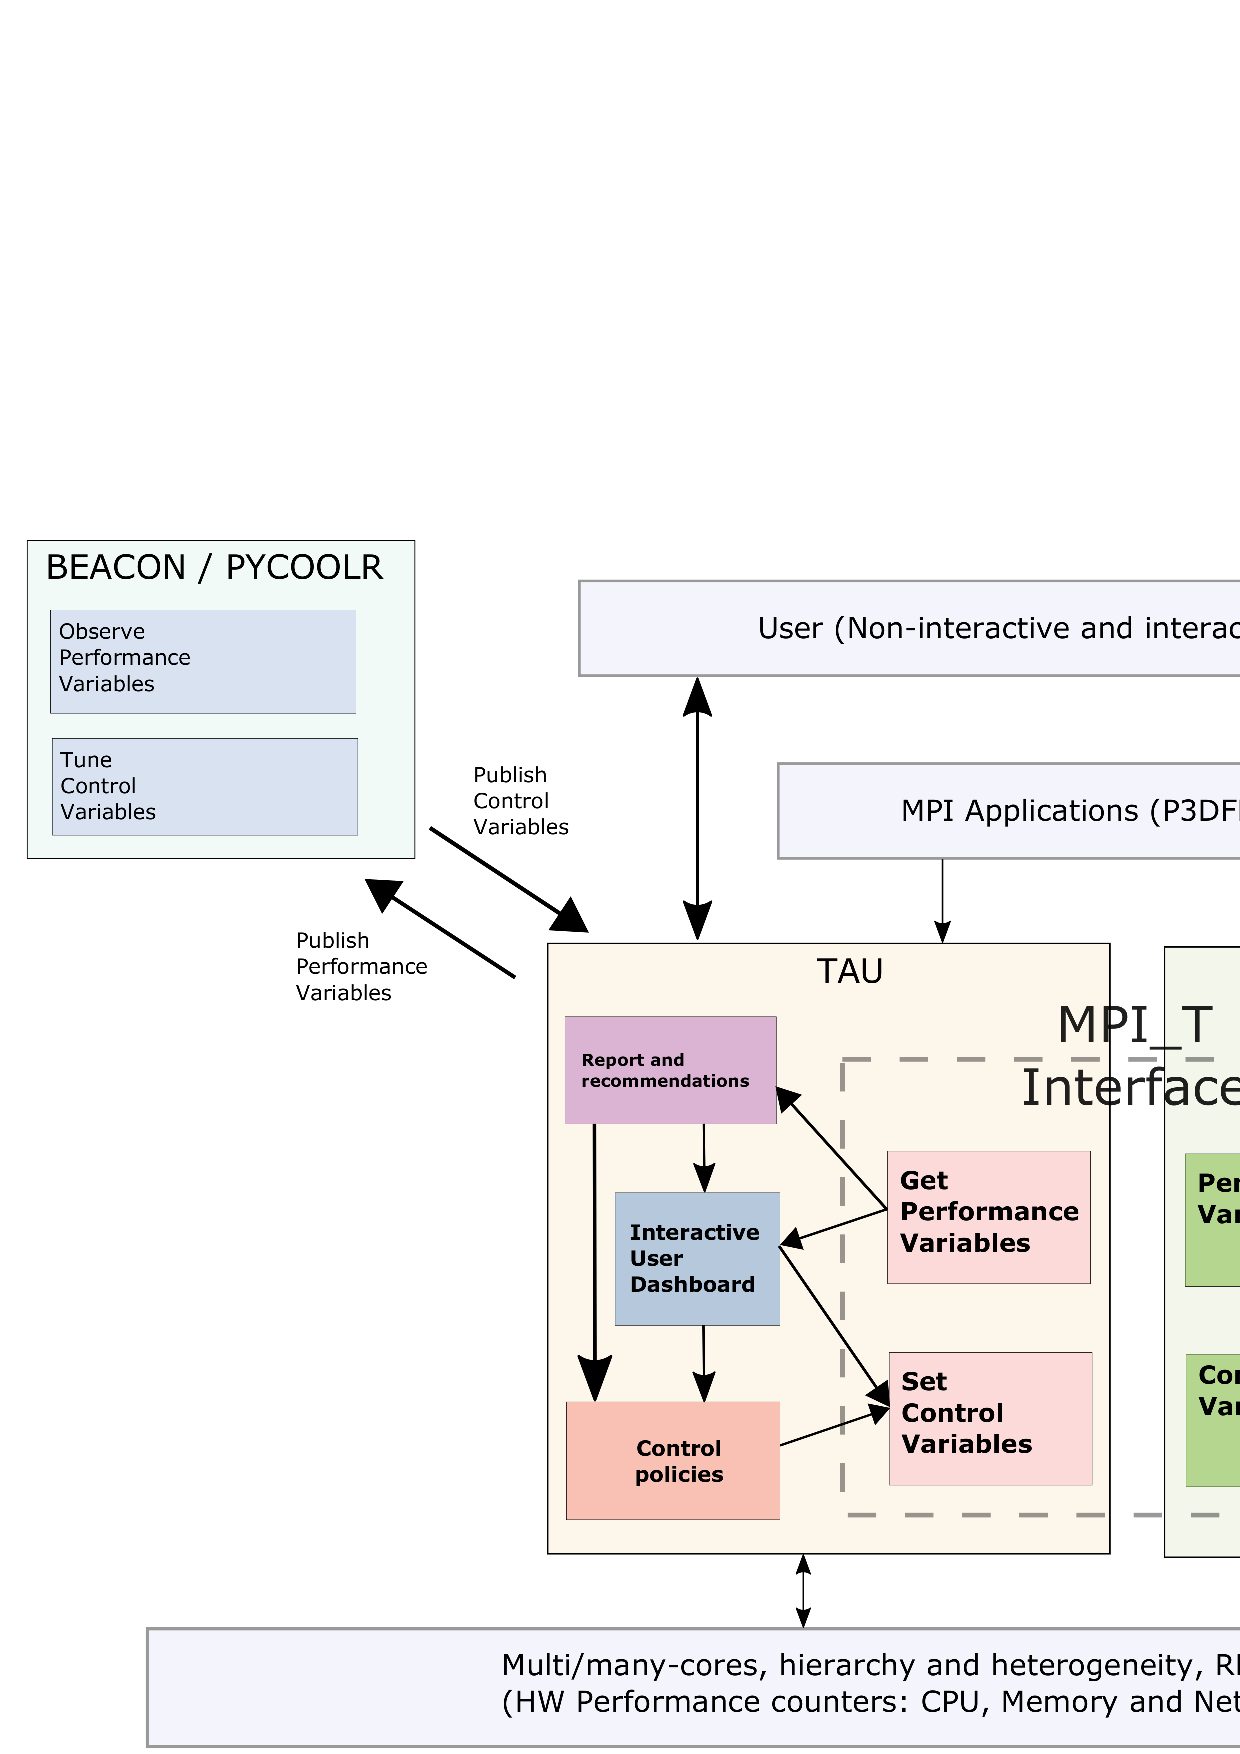
\includegraphics[scale=0.3, width=\columnwidth, keepaspectratio]{figures/MPI_T_infrastructure}
		\caption{Integrated MVAPICH2 and TAU infrastructure based on MPI\_T}
		\label{fig:mpitinfrastructure}
	\end{figure*}
\end{center}

\subsection {Monitoring and Controlling Usage of Virtual Buffers} 
Virtual Buffers (VBUFs) are used in MVAPICH2 to temporarily store messages in transit between two processes. The use of virtual buffers can offer significant performance improvement to applications performing heavy point-to-point communication, such as stencil-based codes. MVAPICH2 offers a number of PVARs that monitor the current usage level, availability of free VBUFs in different VBUF pools, maximum usage levels, and the number of allocated VBUFs at process level granularity. Accordingly, it exposes CVARs that modify how MVAPICH2 allocates and frees these VBUFs at runtime.

\section{Enabling Runtime Instrospection and Online Monitoring}
MPI\_T makes it possible to inquire about the state of the underlying MPI implementation through the query of performance variables. While it is the prerogative of the MPI implementation what PVARs are published, the tool must be extended to use MPI\_T for access. Similarly, control variables are defined by the MPI implementation but set by the tool using MPI\_T. Below we discuss how this is done in TAU to realize introspection and tuning.
\subsection{Gathering Performance Data}
TAU has been extended to support the gathering of performance data exposed through the MPI\_T interface. Each tool that is interested in querying MPI\_T must first register a \textit{performance session} with the interface. This object allows the MPI library to store separate contexts and differentiate between multiple tools/components that are simultaneously querying the MPI\_T interface. Along with a \textit{performance session}, a tool must also allocate \textit{handles} for all the performance variables that it wishes to read/write. Within TAU, the task of allocating the global (per-process) performance session and handles for PVARs is carried out inside the TAU tool initialization routine. However, this design has a caveat --- an MPI library can export additional PVARs during runtime as they become available through dynamic loading. A tool must accordingly allocate handles for these additional PVARs if it wishes to read them. TAU currently does not support this --- we are restricted to reading PVARs that are exported at TAU initialization. We plan to support the dynamic use case in a future release.
\par TAU can use sampling to collect performance variables periodically. When an application is profiled with TAU's MPI\_T capabilities enabled, an interrupt is triggered at regular intervals. Inside the signal handler for the \verb+SIGALRM+ signal, the MPI\_T interface is queried and the values of \textit{all} the performance variables exported are stored at process level granularity. TAU registers internal \textit{atomic user events} for each of these performance variables, and every time an event is triggered (while querying the MPI\_T interface), the running average, minimum value, the maximum value, and other basic statistics are calculated and available to the user at the end of the profiling run. These statistics carry meaning only for PVARs that represent \verb+COUNTERS+ or \verb+TIMERS+. Thus, we define TAU user events to store and analyze PVARs for these two classes. The MPI\_T interface allows MPI libraries to export PVARs from a rich variety of classes --- timers, counters, watermarks, state information, and so on. MVAPICH2 and TAU have been primarily designed to support PVARs from the \verb+TIMER+ or \verb+COUNTER+ classes. As part of future work, we plan to export a richer variety of PVAR classes and design appropriate methods for storage and analysis of each of these classes.
\par TAU also provides an application-level API to query all exported PVARs as and when the application desires (i.e., in a synchronous manner). However, we have chosen not to demonstrate this method of sampling PVARs in our experiments.

\subsection{Online Monitoring}
Runtime introspection naturally extends to online monitoring where certain performance variables are made viewable during execution. Figure \ref{fig:onlinemonitoringdesign} depicts the interaction between TAU and BEACON to enable online monitoring of PVARs through the PYCOOLR GUI.
\par To interface TAU and BEACON, TAU defines a BEACON \textit{topic} for performance variables and publishes PVAR data collected at runtime to this topic. Any software component interested in monitoring PVARs can then subscribe to this topic and receive live updates for all performance variables exported by the MPI implementation.
\par To monitor PVARs on PYCOOLR, the PYCOOLR GUI acts as a subscriber to the PVAR topic --- thus it receives updated values for all PVARs from TAU's sampling-based measurement module. The GUI has been extended to offer the user the ability to select only those PVARs that he/she is interested in monitoring --- this is a useful feature as an MPI library can export 100's of PVARs, not all of which may interest the user. The GUI plots the values for the selected PVARs at runtime as and when it receives them through BEACON.

\subsection{Viewing Performance Data}
ParaProf is the TAU component that allows the user to view and analyze the collected performance profile data post-execution. This profile information is collected on a per-thread or a per-process level, depending on whether or not threads were used in the application. ParaProf has existing support for the analysis of \textit{interval events} as well as \textit{atomic user events}. Interval events are used to capture information such as the total execution time spent inside various application routines. Atomic user events are used to store information such as hardware counter values. 
\par PVARs are treated as atomic user events. ParaProf's existing support for analyzing atomic user events has been leveraged to display PVAR data for each process. Performance variables collected from the MPI\_T interface during execution are displayed on ParaProf as events that include markers indicating high variability.

\begin{center}
        \begin{figure*}[tbp!]
        \centering
                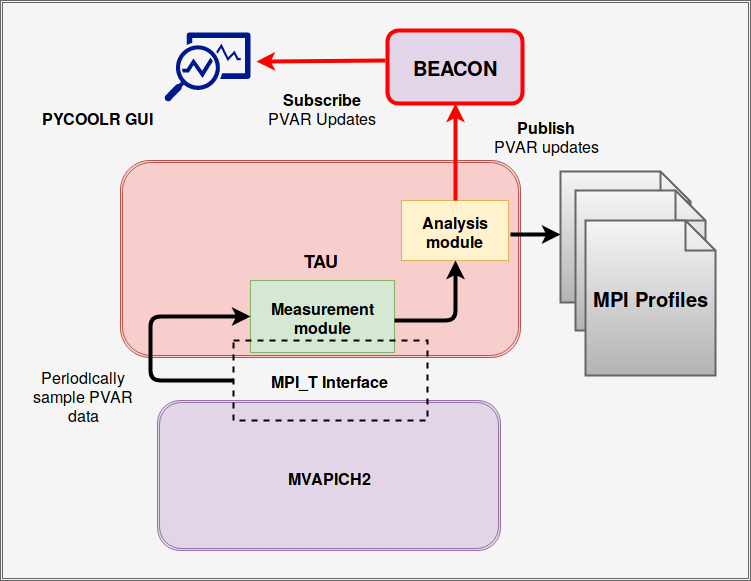
\includegraphics[scale=0.35,keepaspectratio]{figures/Online_Monitoring_Design}
                \caption{Online monitoring with BEACON/PYCOOLR}
                \label{fig:onlinemonitoringdesign}
        \end{figure*}
\end{center}

\section{Runtime Tuning through MPI\_T}
Complementary to providing an API for runtime introspection, the MPI\_T interface also enables a mechanism to modify the behavior of the MPI library through control variables. MPI implementations can define control variables for configuration, performance, or debugging purposes. MPI libraries may implicitly restrict the semantics of \textit{when} CVARs can be set --- some may be set only once before \verb+MPI_Init+, and others may be set anytime during execution. Further, there may be restrictions on whether or not CVARs are allowed to have different values for different processes --- this decision is left entirely up to the MPI library. Therefore, a tool or a user interacting with the MPI\_T interface for the purpose of tuning the MPI library must be aware of the particular semantics associated with the CVARs of interest.
\subsection {User-Guided Tuning through PYCOOLR} Our infrastructure provides users the ability to fine-tune the MPI library by setting CVARs at runtime. As depicted in Figure \ref{fig:manualtuning}, we use the BEACON backplane communication infrastructure to enable user-guided tuning. TAU and BEACON interface with each other in a bi-directional fashion. Aside from acting as a publisher of PVAR data, TAU is a subscriber to a BEACON topic used for communicating CVAR updates. The PYCOOLR GUI has been extended to enable the user to set new values for multiple CVARs at runtime --- Figure \ref{fig:pycoolrcvars} displays a screenshot of the PYCOOLR window that enables this functionality.
\par Together with the online monitoring support provided by PYCOOLR, this user-guided tuning infrastructure can enable a user to experiment with different settings for CVARs and note their effects on selected PVARs or other performance metrics. We must note that this infrastructure has one significant limitation --- the value that the user sets for a CVAR is \textit{uniformly} applied across MPI processes. In other words, each MPI process receives the same value for the CVAR --- this may not be ideal, as it is likely that each process displays a different behavior and thus may have a different optimal value for a given setting. We argue that this infrastructure is nevertheless useful in the experimentation phase, wherein the user is trying to determine the CVAR that is important for a given situation/application.

\begin{center}
        \begin{figure*}[tbp!]
        \centering
                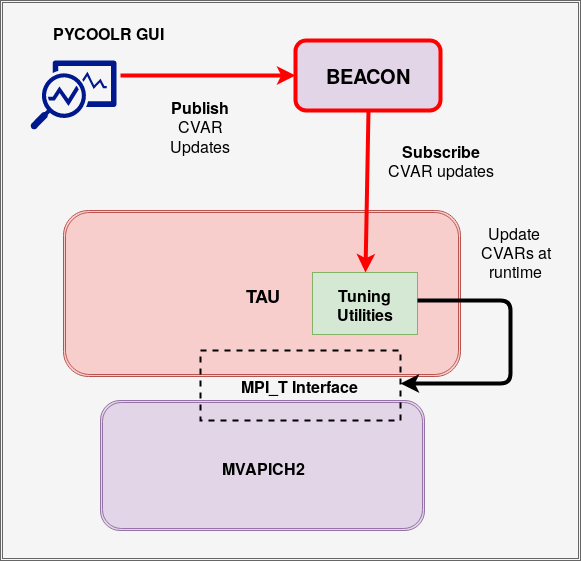
\includegraphics[scale=0.4,keepaspectratio]{figures/Manual_Tuning_Design}
                \caption{User-guided tuning with BEACON/PYCOOLR}
                \label{fig:manualtuning}
        \end{figure*}
\end{center}

\subsection{Plugin Infrastructure in TAU}

TAU is a comprehensive software suite that is comprised of well-separated components providing instrumentation, measurement and analysis capabilities. Our vision for performance engineering of MPI applications involves a \textit{more active} involvement of TAU in monitoring, debugging and tuning behavior \textit{at runtime}. The MPI\_T interface provides tools an opportunity to realize this vision.
\par Recall that the MPI\_T interface allows MPI implementations complete freedom in defining their own PVARs and CVARs to export. However, this freedom comes with a cost to tool writers for MPI\_T --- each MPI implementation will require its own custom tuning and re-configuration logic. From a software infrastructure development standpoint, it would be preferable to design a framework that will allow multiple such customized autotuning logic to co-exist \textit {outside of core tool logic}, and be appropriately loaded depending on the MPI library being used. With this motivation in mind, we have added support for a \textit{generic} plugin infrastructure in TAU that can be used to develop and load custom logic for a variety of performance engineering needs. The latest version of TAU supports this plugin infrastructure.

\begin{center}
        \begin{figure}[tbp!]
         \centering
         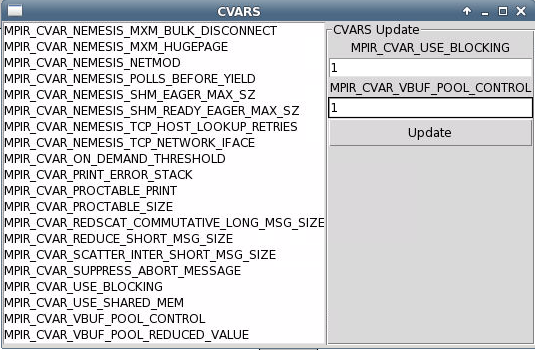
\includegraphics[scale=0.5,keepaspectratio]{figures/Pycoolr-CVARs}
         \caption{Screenshot of PYCOOLR window to update CVARs}
         \label{fig:pycoolrcvars}
        \end{figure}
\end{center}

\subsubsection{Design Overview} In the current design, plugins are \verb+C/+\verb+C+\texttt{++} modules that are built into separate shared libraries (Dynamic Shared Objects). The path to the directory containing the plugins is specified using the environment variable \verb+TAU_PLUGINS_PATH+. The list of plugins to be dynamically loaded at runtime is specified using the environment variable \verb+TAU_PLUGINS+ separated by a colon as a delimiter. 
\par In keeping with the general design of plugin frameworks, the TAU plugin system has the following stages:
\begin {itemize}
\item \textbf{Initialization}: This is invoked during TAU library initialization. During this phase, TAU's plugin manager reads the environment variables \verb+TAU_PLUGINS_PATH+ and \verb+TAU_PLUGINS+ and loads the plugins in the order specified by \verb+TAU_PLUGINS+. Each plugin \textit{\textbf{must}} implement a function called \verb+Tau_plugin_init_func+. Inside this function, it can register callbacks for a subset of \textit{plugin events} it is interested in. Note that each plugin may register callbacks for more than one event. The plugin manager maintains an \textit{ordered} list of active plugins for each event supported.
\item \textbf{Event Callback Invocation}: We define some salient plugin events in TAU that could be interesting or useful from a performance engineering standpoint. These events are discussed in detail in the section that follows. When these plugin events occur during execution of an application instrumented with TAU, the plugin manager invokes the registered callbacks for the specific event in the order in which the corresponding plugins were loaded. Each event that is supported has a specific, typed data object associated with it. When the event occurs, this data object is populated and sent as a parameter to the plugin callback. 
\item \textbf{Finalize Phase}: When TAU is done generating the profiles for the application, the plugins are unloaded, and all the auxiliary memory resources allocated by the plugin manager are freed.
\end{itemize}

\subsubsection{Plugin Events Supported}
Plugin events are entry points into the plugin code that performs a custom task. Currently, TAU defines and supports the following events:
\begin{itemize}
\item \verb+TAU_PLUGIN_EVENT_FUNCTION_REGISTRATION+: TAU creates and registers a \verb+FunctionInfo+ object for all functions it instruments and tracks. This event marks the end of the registration phase for the \verb+FunctionInfo+ object that was created.
\item \verb+TAU_PLUGIN_EVENT_ATOMIC_EVENT_REGISTRATION+: TAU defines \textit{atomic events} to track PAPI counters, PVARs and other entities which do not follow interval event semantics. This plugin event marks the end of the registration phase for the atomic event and is triggered when the atomic event is created. In the context of our MPI\_T infrastructure, this plugin event is triggered once for every PVAR that is exported by the MPI library.
\item \verb+TAU_PLUGIN_EVENT_ATOMIC_EVENT_TRIGGER+: When the value of an atomic event is updated, this event is triggered. This plugin event is triggered once for each PVAR, every time the MPI\_T interface is queried.
\item \verb+TAU_PLUGIN_EVENT_INTERRUPT_TRIGGER+: TAU's sampling subsystem relies on installing an interrupt handler for the \verb+SIGALRM+ signal, and performs the sampling within this interrupt handler. When TAU is used with its sampling capabilities turned on, this plugin event is triggered within TAU's interrupt handler (10 seconds is the default interrupt interval).
\item \verb+TAU_PLUGIN_EVENT_END_OF_EXECUTION+: When TAU has finished creating and writing the profile files for the application, this plugin event is triggered.
\end{itemize}
There may be other supported events added in future releases.

\subsubsection{Use Case: Filter Plugin to Disable Instrumentation at Runtime}
To demonstrate a sample usage scenario for the plugin architecture, we have created a plugin that filters out instrumented functions from being profiled at runtime, based on a user-provided selective instrumentation file. This situation arises when the application has been instrumented using either the compiler or TAU's source instrumentation tool --- the Program Database Toolkit (PDT)~\cite{PDT}.
\par PDT works by parsing the input source file to detect function definitions and function call sites, and automatically adds the TAU instrumentation API calls to these sites. The user may want to prevent certain \textit{automatically instrumented functions} from being profiled --- these functions may be frequently invoked but not have a significant impact on overall runtime. They may pollute the generated profiles and more importantly, add to the measurement overheads without providing any real benefit. From a profiling standpoint, there is solid motivation to provide a mechanism that allows such functions to be excluded from profiling.
\par We use our plugin infrastructure to provide this functionality --- our filter plugin registers a callback for the \verb+TAU_PLUGIN_EVENT_FUNCTION_REGISTRATION+ plugin event. Recall that this event is triggered once for every function instrumented by TAU. Within the callback for the \\\verb+TAU_PLUGIN_EVENT_FUNCTION_REGISTRATION+ event, we read a user-provided selective instrumentation file that contains a list of functions to be excluded from profiling. The data object for this plugin event contains the function name information. If there is a match between the function being registered and the list of function names in the selective instrumentation file, we set the profile group for the function to be \verb+TAU_DISABLE+, effectively switching off profiling for this function.

\subsection{Plugins for Autotuning}
Figure \ref{fig:plugininfrastructure} depicts TAU plugins in the context of our MPI\_T infrastructure. As discussed earlier, TAU samples PVAR data from the MPI\_T interface inside a signal handler for the \verb+SIGALRM+ signal. TAU can use this collected PVAR data to perform an autotuning decision inside the signal handler --- this is realized through plugins that install callbacks for the \verb+TAU_PLUGIN_EVENT_INTERRUPT_TRIGGER+ event. This event is triggered every time TAU samples the MPI\_T interface, and the registered plugin callbacks are invoked. Inside the callback, the plugin has access to all the PVAR data collected and performs a \textit{runtime autotuning decision} that may result in updated values for \textit{one or more} CVARs (knobs). Plugins can make use of core TAU modules to interact with the MPI\_T interface to update CVAR values.
\par Note that the plugin infrastructure allows the user to specify more than one plugin --- this feature can be utilized to load multiple autotuning policies, each of which is built into a separate shared library. While plugins use common functionality defined inside TAU to read or write to the MPI\_T interface, the autotuning logic itself is custom to each plugin --- in the future, we plan to support a high-level infrastructure to express autotuning policies that reduce duplicated code across plugins. Our starting point for developing autotuning policies relies on users with background or offline knowledge about specific domains, applications, and libraries.

\begin{center}
        \begin{figure*}[tbp!]
         \centering
                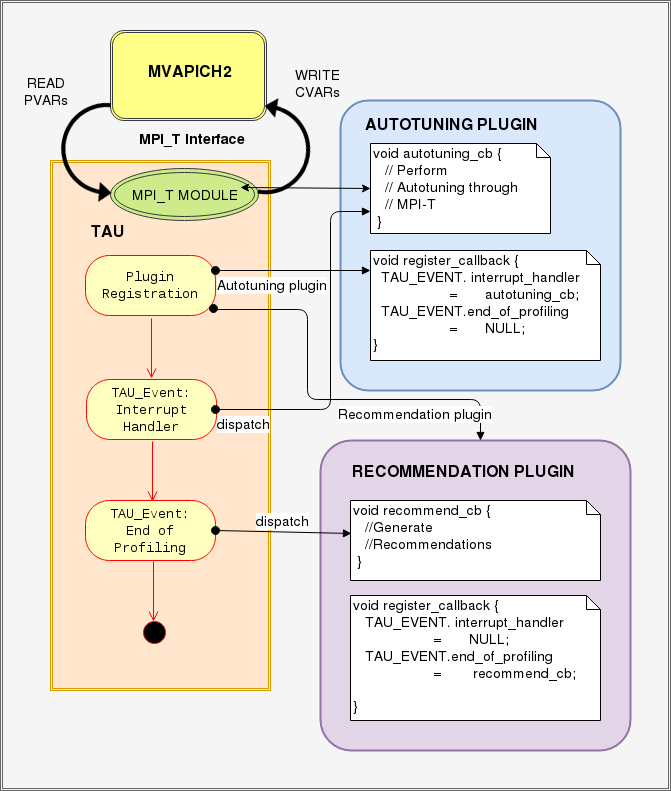
\includegraphics[scale=0.5,width=\columnwidth,keepaspectratio]{figures/Plugin_Infrastructure}
                \caption{Plugin infrastructure}
                \label{fig:plugininfrastructure}
        \end{figure*}
\end{center}

\subsection{Plugins for Recommendations}
We take advantage of the plugin mechanism to develop performance recommendations for the user. MPI libraries can export a large number of control variables --- many of which are also environment variables whose default settings may not always be optimal for a given application/situation. Moreover, the user may not even be aware of the existence of certain settings or MPI implementation-specific features that can improve performance. A profiling tool such as TAU is in an ideal position to fill this gap with the MPI\_T interface acting as an enabling mechanism. \par Performance data gathered by TAU through the MPI\_T and PMPI interface can be analyzed by a recommendation plugin to provide useful hints to the user at the end of the application execution. Recommendation plugins register callbacks for the \verb+TAU_PLUGIN_EVENT_END_OF_EXECUTION+ event that is triggered when TAU has finished collecting and writing profile information. Currently, TAU supports the generation of recommendations as part of the metadata that is associated with each process. This metadata is available for viewing on ParaProf.


\section{Target Applications}
  \subsection{AmberMD}

  AmberMD~\cite{AmberMD} is a popular software package that consists of tools to carry out molecular dynamics simulations. A core component is the molecular dynamics engine, \verb+pmemd+, which comes in two flavors: serial and an MPI parallel version. We focus on improving the performance of molecular dynamics simulations that use the parallel MPI version of \verb+pmemd+. A substantial portion of the total runtime is attributed to MPI communication routines, and among MPI routines, calls to \verb+MPI_Wait+ dominate in terms of contribution to runtime. However, in terms of number of MPI calls made, \verb+MPI_Isend+ and \verb+MPI_Irecv+ dominate. The use of non-blocking sends and receives explicitly allows the opportunity for a greater communication-computation overlap.
  \subsection{SNAP}
  SNAP~\cite{SNAP} is a proxy application from the Los Alamos National Laboratory that is designed to mimic the performance characteristics of PARTISN~\cite{PARTISN}. PARTISN is a neutral particle transport application that solves the linear Boltzmann transport equation for determining the number of neutral particles in a multi-dimensional phase space. SNAP is considered to be an updated version of the Sweep3D~\cite{Sweep3D} proxy application and can be executed on hybrid architectures. SNAP heavily relies on point-to-point communication, and the size of messages transferred is a function of the number of spatial cells per MPI process, number of angles per octant, and number of energy groups. \par
  Specifically, a bulk of the point-to-point communication is implemented as a combination of \verb+MPI_Isend+/\verb+MPI_Waitall+ on the sender side, and \verb+MPI_Recv+ on the receiver side. This explicitly allows the opportunity for communication-computation overlap on the sender side. 
  \subsection{3DStencil}
  We designed a simple synthetic stencil application that performs non-blocking point-to-point communication in a cartesian grid topology. In between issuing the non-blocking sends and receives and waiting for the communication to complete, the application performs arbitrary computation for a period of time that is roughly equal to the end-to-end time for pure communication alone. The goal is to evaluate the degree of communication-computation overlap. In an ideal scenario of 100\% overlap, the computation would complete at the same time as communication, so that no additional time is spent in waiting for the non-blocking communication requests to complete. For the purposes of this experiment, point-to-point communication involves messages of an arbitrarily high, but fixed size. 
 \subsection{MiniAMR}

  MiniAMR is a mini-app that is a part of the Mantevo~\cite{Mantevo} software suite. As the name suggests, it involves adaptive mesh refinement and uses 3D Stencil computation. MiniAMR is a memory bound application, and communication time is dominated by \verb+MPI_Wait+ for point-to-point routines involving small messages (1-2 KB range) and \verb+MPI_Allreduce+. The \verb+MPI_Allreduce+ call involves messages of a constant, small size (8 bytes) making it latency sensitive. This call is part of the check-summing routine and increasing the check-summing frequency or the number of stages per timestep impacts the scalability of this routine and thus the application.

\section{Usage Scenarios}
MPI\_T in combination with the TAU plugin architecture makes it possible to do powerful operations that would be difficult to realize otherwise. The following describes the design of a recommendation to enable hardware offloading of collectives, and an autotuning policy to free unused MPI internal buffers using MPI\_T. These policies are implemented using plugins.
\subsection{Recommendation Use Case: Hardware Offloading of Collectives}
MVAPICH2 now supports offloading of \verb+MPI_Allreduce+ to network hardware using the SHArP~\cite{SHARP} protocol. Hardware offloading is mainly beneficial to applications where communication is sensitive to latency. As the \verb+MPI_Allreduce+ call in MiniAMR involves messages of 8 bytes, it is a prime candidate to benefit from hardware offloading. \par
During the profiling phase, TAU collects statistics about the average message size involved in \verb+MPI_Allreduce+ operation. It also collects the time spent within \verb+MPI_Allreduce+ versus the overall application time. If the message size is below a certain threshold and the percentage of total runtime spent within \verb+MPI_Allreduce+ is above a certain threshold, through ParaProf, TAU recommends the user to set the CVAR \verb+MPIR_CVAR_ENABLE_SHARP+ for subsequent runs. Note that this recommendation policy was implemented using plugins. The same infrastructure can be used to support multiple recommendation policies.
\subsection{Autotuning Use Case: Freeing Unused Buffers}
MVAPICH2 uses internal communication buffers (VBUFs) to temporarily hold messages that are yet to be transferred to the receiver in point-to-point communications. There are multiple VBUF pools which vary in size of the VBUF. At runtime, MVAPICH2 performs a match based on the size of the message and accordingly selects a VBUF pool to use. Specifically, these VBUFs are used when MVAPICH2 chooses to send the message in an \emph{Eager} manner to reduce communication latency. Typically, short messages are sent using the \emph{Eager} protocol, and longer messages are sent using the \emph{Rendezvous} protocol, which does not involve the use of VBUFs. The primary scalability issue with using \emph{Eager} protocol is excessive memory consumption that can potentially lead to an application crash. \par
Depending on the pattern of message sizes involved in point-to-point communication, the usage level of these VBUF pools can vary with time and between processes. It can be the case that the application makes scarce use of VBUFs, or uses VBUFs only from one pool (3DStencil is one such use case). In such a scenario, unused VBUFs represent wasted memory resource. There could be significant memory savings in freeing these unused VBUFs.

For this use case, specific CVARs include:
\begin{itemize}
  \item \verb+MPIR_CVAR_IBA_EAGER_THRESHOLD+: The value of this CVAR represents the message size above which MVAPICH2 uses the \emph{Rendezvous} protocol for message transfer in point-to-point communication. Below this message size, MVAPICH2 uses the \emph{Eager} protocol
  \item \verb+MPIR_CVAR_VBUF_TOTAL_SIZE+: The size of a single VBUF. For best results, this should have the same value as \verb+MPIR_CVAR_IBA_EAGER_THRESHOLD+
  \item \verb+MPIR_CVAR_VBUF_POOL_CONTROL+: Boolean value that specifies if MVAPICH2 should try to free unused VBUFs at runtime. By default, MVAPICH2 will try to free from any available pool if this variable is set
  \item \verb+MPIR_CVAR_VBUF_POOL_REDUCED_VALUE+: This CVAR specifies the lower limit to which MVAPICH2 can reduce the number of VBUFs. This is an array, and each index represents the corresponding VBUF pool. This CVAR takes effect only if  pool control is enabled. This CVAR allows more fine-grained control over freeing of VBUFs, potentially reducing unnecessary allocations and freeing of VBUFs, if the usage pattern is known in advance
\end{itemize}

Correspondingly, PVARs of interest include:
\begin{itemize}
  \item \verb+mv2_vbuf_allocated_array+: Array that represents the number of VBUFs allocated in a pool specified by an index
  \item \verb+mv2_vbuf_max_use_array+: Array that represents the maximum number of VBUFs that are actually used in a given pool specified by an index
  \item \verb+mv2_total_vbuf_memory+: Total VBUF memory (in bytes) used for the specified process across all pools
\end{itemize}

\subsubsection{Autotuning Policy}
When we increase the value of the \emph{Eager} limit specified by \verb+MPIR_CVAR_IBA_EAGER_THRESHOLD+, there is an opportunity for increased overlap between communication and computation as larger messages are sent eagerly. As a result, the overall execution time for the application may reduce. Figure \ref{fig:beforeeager} is an enlarged Vampir~\cite{Vampir} summary process timeline view for one iteration of the 3DStencil application before applying the Eager optimization. Figure \ref{fig:aftereager} is a Vampir summary process timeline view for one iteration of the 3DStencil application after applying the Eager optimization. The timeline view focuses on the phase of the iteration where there is an explicit opportunity for communication-computation overlap through the use of non-blocking sends and receives. The X-axis represents time and the Y-axis represents the percentage of MPI processes inside user code (green) and MPI code (red) respectively at any given instant in time --- larger areas of green indicates a higher amount of useful work (computation) performed by processes as a result of a larger communication-computation overlap. 

 \begin{figure*}[tbp!]
  \centering
  \captionsetup{justification=centering}
  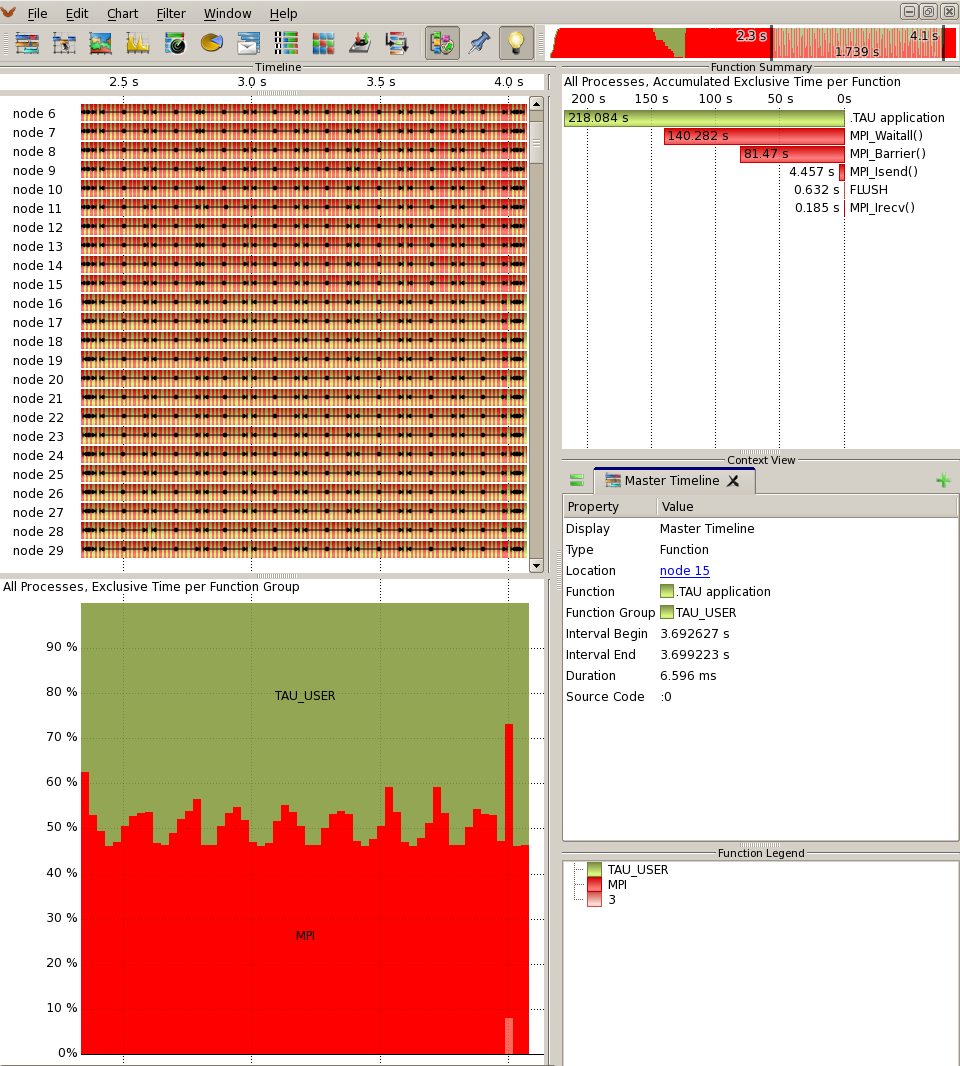
\includegraphics[scale=1.0,width=\columnwidth,keepaspectratio]{figures/Overlap-before}
         \caption{Vampir summary process timeline view of 3DStencil before Eager threshold tuning}
 \label{fig:beforeeager}
 \end{figure*}

 \begin{figure*}[tbp!]
  \centering
  \captionsetup{justification=centering}
  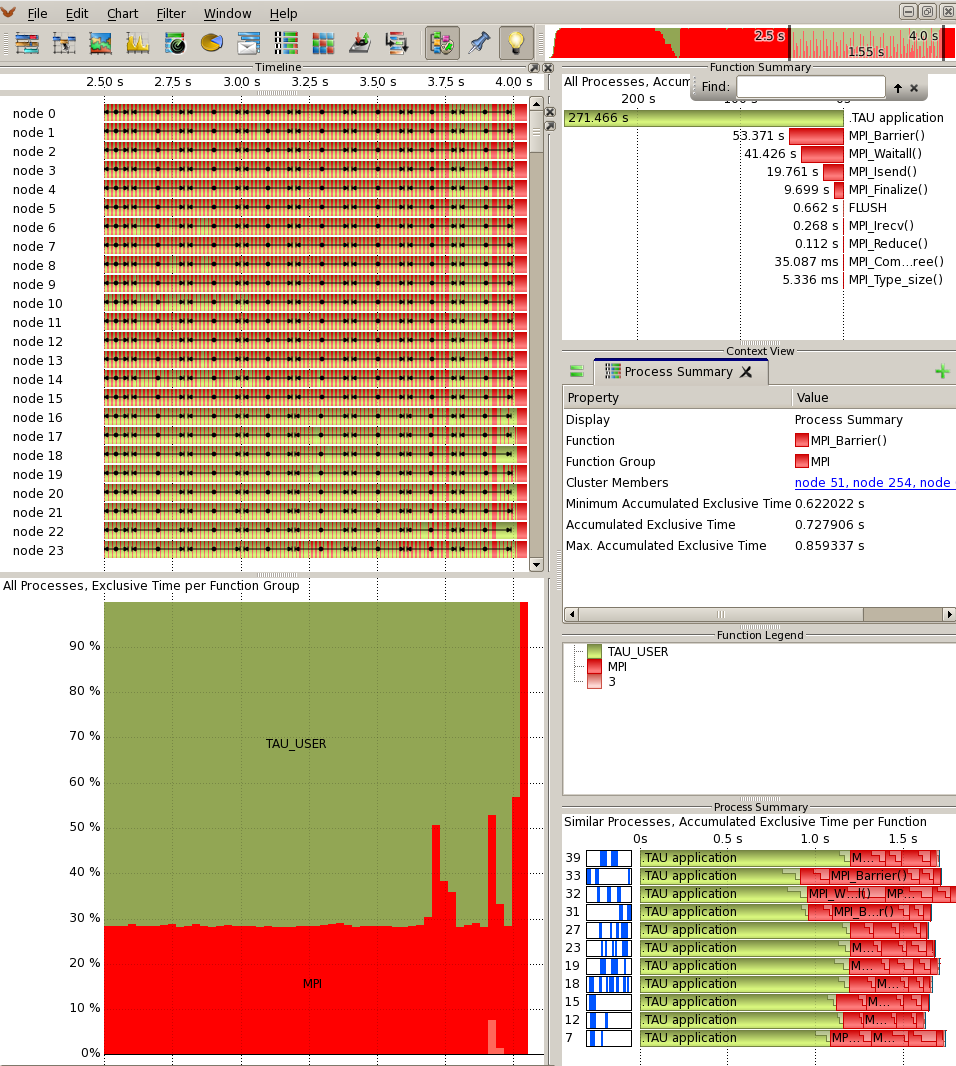
\includegraphics[scale=1.0,width=\columnwidth,keepaspectratio]{figures/Overlap-after}
         \caption{Vampir summary process timeline view of 3DStencil after Eager threshold tuning: increased time spent in user code}
 \label{fig:aftereager}
 \end{figure*}


\par Figure \ref{fig:aftereager} shows the effect of an increased Eager threshold --- a 20\% increase in the number of MPI processes inside user code during the phase where communication is overlapped with computation. This increase is due to the fact that less time is spent waiting for the non-blocking calls to complete at the \verb+MPI_Wait+ barrier. With a larger eager threshold, the MPI library can advance communication in the background while the sending process is busy performing the computation. The extreme right edges of Figure \ref{fig:aftereager} are to be ignored as they represent the phase where the application is performing pure communication.\par
Increasing the Eager limit may have the following two distinct effects:
\begin{itemize}
\item Larger VBUFs may need to be allocated. Note that this does not mean that \textit{more} VBUFs are allocated --- it only means that the size of each individual VBUF in the affected pool has increased in order to hold larger messages. Recall that MVAPICH2 has four VBUF pools --- the VBUFs from different pools vary in only their size. 
\item As a result of the increased Eager limit, larger messages would be transferred through the Eager protocol instead of the Rendezvous protocol. Depending on the communication characteristics of the application, this may lead to increased usage of VBUFs from one or more VBUF pools. If there is a shortage of VBUFs in a given pool, MVAPICH2 may need to allocate additional VBUFs.
\end{itemize}

A combination of these two factors may lead to an increase in the total VBUF memory usage inside MVAPICH2. Figure \ref{fig:pycoolrincr} is a PYCOOLR screenshot illustrating this increase in total VBUF memory usage (across all four pools) for AmberMD application when the Eager threshold is raised. We see a similar increase in total VBUF memory usage for the 3DStencil application as well. The X-axis represents time and the Y-axis represents memory in bytes with 10\textsuperscript{7} as the multiplier. Each red dot represents the instantaneous \verb+mv2_total_vbuf_memory+ (in bytes) for one MPI process. If MPI processes have the same VBUF memory usage at any point in time, then the red dots would overlap. From Figure \ref{fig:pycoolrincr}, it is evident that there are two classes of processes --- one with a VBUF memory usage of roughly 3 MB (before Eager tuning), and another with a VBUF memory usage level of roughly 6 MB (before Eager tuning). The eager threshold is raised by setting the CVAR \verb+MPIR_CVAR_IBA_EAGER_THRESHOLD+ and \verb+MPIR_CVAR_VBUF_SIZE+ statically, during \verb+MPI_Init+. Figure \ref{fig:pycoolrincr} shows that the \verb+mv2_total_vbuf_memory+ increases to approximately 12 MB for the processes with a lower VBUF memory usage, and approximately 23 MB for the class of processes with a higher VBUF memory usage.

\par While one pool sees an increase in VBUF usage, it is possible that other VBUF pools may have unused VBUFs that can be freed to partially offset this increased memory usage inside MPI. In applications such as 3DStencil or AmberMD where the message size is fixed or in a known range, VBUFs from only one pool is used. In such a scenario, freeing unused VBUFs from other pools leads to significant memory savings. The usage levels of VBUF pools would vary from one application to another depending on the particular characteristics of the point-to-point communication. \par
MPI\_T offers a mechanism to monitor pool usage at runtime. Our autotuning policy implemented as a plugin monitors the difference between the \textit{array} PVARs \verb+mv2_vbuf_allocated_array+ and \verb+mv2_vbuf_max_use_array+ --- each pool has a unique ID, and this unique ID is used to index into these two arrays. The difference between these two quantities at a given pool index represents the quantity of wasted memory resource in that pool. If this difference breaches a user-defined threshold for at least one pool, the autotuning policy sets the CVAR \verb+MPIR_CVAR_VBUF_POOL_CONTROL+ to enable MVAPICH2 to free any unused VBUFs. In order to enable more fine-grained control over freeing of unused VBUFs, MVAPICH2 exports an \textit{array} CVAR \verb+MPIR_CVAR_VBUF_POOL_REDUCED_VALUE+. This CVAR is used to communicate the minimum number of VBUFs that must be available in each pool after enabling pool control. When the threshold for unused VBUFs is breached for at least one pool, the autotuning plugin enables pool control and simultaneously sets this array CVAR to be equal to the array PVAR \verb+mv2_vbuf_max_use_array+ --- this is a heuristic that is employed to determine the new values for the various VBUF pool sizes. If on the other hand, this threshold is not breached for \textit{any} pool, the TAU autotuning plugin unsets the CVAR \verb+MPIR_CVAR_VBUF_POOL_CONTROL+ effectively turning off further attempts to free unused VBUFs by MVAPICH2 until the next time the threshold is breached.\par 
Alternatively, both these CVARs can be set at runtime through the PYCOOLR GUI as well --- however, the advantage of using an autotuning plugin for this purpose is that these values can be set individually and independently for different processes. It can also be more responsive without incurring the delay of communicating with the PYCOOLR GUI. Setting different CVAR values for different processes is not possible through the PYCOOLR GUI. \par 
Figure \ref{fig:pycoolrdecr} depicts the decrease in \verb+mv2_total_vbuf_memory+ for AmberMD when only \verb+MPIR_CVAR_VBUF_POOL_CONTROL+ is enabled through the PYCOOLR GUI, instructing MPI to free any unused VBUFs. Note that the autotuning plugin is not employed here. The CVAR for pool control is enabled at around the 150-second mark, and at this point, the VBUF memory usage levels drop as a result of unused VBUFs being freed.
 \begin{figure*}[tbp!]
  \centering
  \captionsetup{justification=centering}
  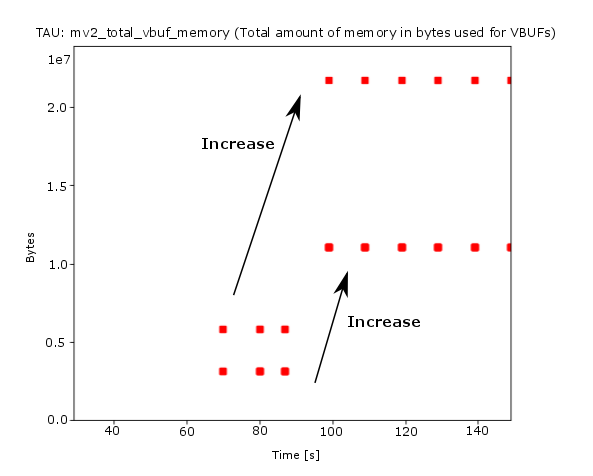
\includegraphics[scale=0.45,keepaspectratio]{figures/Pycoolr-Eager-Part1-plot3-arrows-unblur}
 \caption{PYCOOLR: Increase in total VBUF memory with higher Eager threshold}
 \label{fig:pycoolrincr}
\end{figure*}

 \begin{figure*}[tbp!]
 \centering
  \captionsetup{justification=centering}
 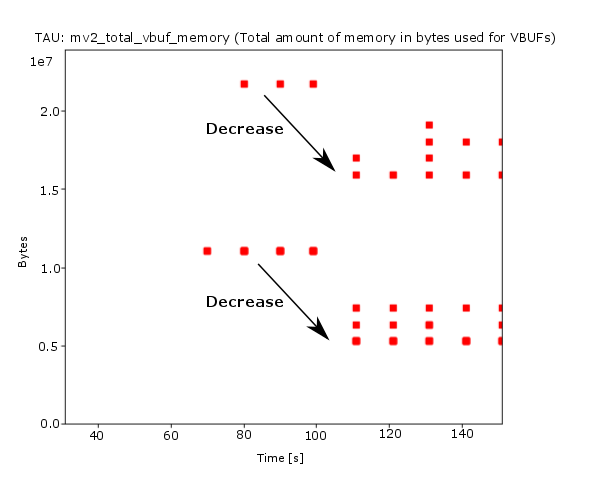
\includegraphics[scale=0.45,keepaspectratio]{figures/Pycoolr-Eager-Part2-plot3-arrows-unblur}
 \caption{PYCOOLR: Decrease in total VBUF memory when freeing unused VBUFs}
 \label{fig:pycoolrdecr}
\end{figure*}

\section{Experiments}
In this section, we present the results obtained from applying the autotuning and recommendation policies to our target applications --- AmberMD, SNAP, 3DStencil, and MiniAMR. We describe results from a study of overheads involved in enabling MPI\_T in MVAPICH2 and TAU.

\subsection{Experimental Setup}
Our experiments with AmberMD, SNAP, and 3DStencil were performed on Stampede, a 6400 node Infiniband cluster at the Texas Advanced Computing Center~\cite{TACC}. Each regular Stampede compute node has two Xeon E5-2680 8-core \quotes{Sandy Bridge} processors and one first-generation Intel Xeon Phi SE10P KNC MIC. We chose to run all our experiments using pure MPI on the Xeon host with 16 MPI processes on a node (1 per core) with \verb+MV2_ENABLE_AFFINITY+ turned on so that MPI tasks were pinned to CPU cores. For SNAP, we used a total of 64 nodes (at 16 processes per node, a total of 1024 processes). For our experiments with AmberMD and 3DStencil, we used a total of 32 nodes (at 16 processes per node, a total of 512 processes). \par
Experiments with MiniAMR and those involving a study of sampling overheads using 3DStencil were performed on the ri2 Infiniband cluster at The Ohio State University. Each compute node on ri2 has two 14-core Intel Xeon E5-2680 v4 processors. The HCA on all nodes in the cluster is the Mellanox CX-4 100 Gigabit adapter. The OFED version used is MLNX\_OFED\_LINUX-4.1-1.0.2.0 and the Linux kernel version is 3.10.0-327.10.1.el7.x86\_64. We ran all our experiments using pure MPI on Intel Xeon hosts with 28 MPI processes on a node (1 per core) and pinned the MPI processes. We used a total of 2-16 nodes (at 28 processes per node, a total of 56 to 448 processes) for our experiments with 3DStencil, and a total of 8 nodes (at 28 processes per node, a total of 224 processes) for experiments with MiniAMR.

\subsection{Results}

\subsubsection{Amber}
Table \ref{tab:Amber} summarizes the results of modifying the \emph{Eager} threshold and applying the runtime autotuning policy for AmberMD.
The threshold is set statically right after MPI initialization, using \verb+MPIR_CVAR_IBA_EAGER_THRESHOLD+.
We noted that increasing the \emph{Eager} threshold from the MVAPICH2 default value to 64000 bytes had the effect of reducing application runtime by 19.2\%. This was achieved at the cost of increasing the total VBUF memory across all processes by 320\%. Please note that the total VBUF memory usage reported here is the \textit{average} value across the number of times that this metric was sampled (once every 10 seconds). The third row shows results of applying the user-defined policy of freeing unused VBUFs at runtime, on top of the \emph{Eager} threshold optimization. We saw a sizeable reduction in total VBUF memory used while the runtime remained unaffected.

\begin{table*}[!bp]
  \centering
  \small
  \captionsetup{justification=centering}
  \caption{AmberMD: Impact of Eager threshold and autotuning on execution time and memory usage}
  \label{tab:Amber}
  \resizebox{\columnwidth}{!}{\begin{tabular}{|c|c|c|c|c|l|}
    \toprule
    Run& \begin{tabular}{@{}c@{}}Number of \\ Processes\end{tabular} & \begin{tabular}{@{}c@{}} Eager \\ Threshold \\ (Bytes)\end{tabular} & Timesteps& \begin{tabular}{@{}c@{}}Runtime \\ (secs)\end{tabular} & \begin{tabular}{@{}c@{}}Total \\ VBUF \\ Memory(KB)\end{tabular}\\
    \midrule
    Default&512&MVAPICH2 Default&8,000&166&4,796,067\\
    Eager&512&64,000&8,000&134&15,408,619\\
    TAU autotuning&512&64,000&8,000&134&15,240,073\\
  \bottomrule
\end{tabular}}
\end{table*}
\subsubsection{SNAP}
SNAP application relies heavily on point-to-point communication, and the message sizes involved in communication depend on a number of input factors. We followed the recommended ranges for these input factors:
\begin{itemize}
\item Number of angles per octant (nang) was set to 50
\item Number of energy groups (ng) was set to 150
\item Number of spatial cells per MPI rank was set to 1200
\item Scattering order (nmom) was set to 4
\end{itemize}
We gathered the message sizes involved in MPI communication. Table \ref{tab:SNAP_profile} lists the five MPI functions that account for the highest aggregate time spent. \verb+MPI_Recv+ and \verb+MPI_Waitall+ together account for nearly 17\% of total application time or 60\% of MPI time. Table \ref{tab:SNAP_message_sizes} lists the message sizes involved in various MPI routines. It is evident that the bulk of messages are point-to-point messages with a message size of roughly 18,300 bytes. \par
The fact that the application spends a lot of its communication time inside \verb+MPI_Recv+ (callsite ID 5 in Table \ref{tab:SNAP_profile}) and \verb+MPI_Waitall+ (callsite ID 16 in Table \ref{tab:SNAP_profile}) suggests that the receiver in the point-to-point communication is generally late as compared to the posting of the corresponding \verb+MPI_Isend+ (callsite ID 1 in Table \ref{tab:SNAP_profile}) operation. As a result of the relatively large message size of 18KB involved in this case, the data is transferred using the Rendezvous protocol \textit{after} the receive is posted --- in this specific context, this data transfer happens when the sender reaches the \verb+MPI_Waitall+ call. Even though there is an opportunity for communication-computation overlap through the use of non-blocking routines, no overlap actually happens in the application because of the conditions necessary for the transfer of large messages using the Rendezvous protocol. \par
By increasing both the inter-node and intra-node Eager threshold to 20KB, the transfer of these point-to-point messages is initiated when the sender posts the \verb+MPI_Isend+ operation. As a result, the application sees an increase in communication-computation overlap, and this manifests itself as a reduction in overall application runtime. The second row of Table \ref{tab:SNAP} summarizes this improvement in performance with 1024 processes --- we note a reduction of 10.7\% in application runtime when increasing the Eager threshold to 20 KB. However, increasing the Eager threshold also meant that the total VBUF memory usage across all processes went up by 12\%. \par
The TAU autotuning plugin ensures that VBUFs from unused pools are freed to offset this increase in total VBUF memory usage. The third row of Table \ref{tab:SNAP} summarizes the reduction in total VBUF memory usage when the TAU autotuning plugin is enabled. It is important to note that the plugin does not disturb application runtime even at this scale.

\begin{table*}[!tbp]
  \centering
  \small
  \captionsetup{justification=centering}
  \caption{SNAP: Aggregate time inside various MPI functions (top five by total time)}
  \label{tab:SNAP_profile}
  \resizebox{\columnwidth}{!}{\begin{tabular}{|c|c|c|l|}
    \toprule
    MPI routine name&\begin{tabular}{@{}c@{}}Callsite ID \end{tabular} &  \begin{tabular}{@{}c@{}}Portion of \\ Application Runtime (\%)\end{tabular} & \begin{tabular}{@{}c@{}} Portion of MPI Time (\%)\end{tabular}\\
    \midrule
    MPI\_Recv&4&13.31&47.50\\
    MPI\_Barrier&5&5.20&18.55\\
    MPI\_Allreduce&7&3.84&13.72\\
    MPI\_Waitall&16&3.09&11.02\\
    MPI\_Isend&1&1.21&4.33\\
  \bottomrule
\end{tabular}}
\end{table*}

\begin{table*}[!tbp]
  \centering
  \small
  \captionsetup{justification=centering}
  \caption{SNAP: Average sent message sizes from various MPI functions (top five by message count)}
  \label{tab:SNAP_message_sizes}
  \resizebox{0.80\columnwidth}{!}{\begin{tabular}{|c|c|c|l|}
    \toprule
    MPI routine name&\begin{tabular}{@{}c@{}}Callsite ID \end{tabular} & \begin{tabular}{@{}c@{}}Count\end{tabular} & \begin{tabular}{@{}c@{}} Average Message Size (Bytes)\end{tabular}\\
    \midrule
    MPI\_Isend&1&114348672&18300\\
    MPI\_Allreduce&7&25600&1200\\
    MPI\_Send&18&2400&1920\\
    MPI\_Bcast&11&1024&120\\
    MPI\_Bcast&15&1024&120\\
  \bottomrule
\end{tabular}}
\end{table*}

\begin{table*}[!tbp]
  \centering
  \small
  \captionsetup{justification=centering}
  \caption{SNAP: Impact of Eager threshold and autotuning on execution time and memory usage}
  \label{tab:SNAP}
  \resizebox{\columnwidth}{!}{\begin{tabular}{|c|c|c|c|l|}
    \toprule
    Run& \begin{tabular}{@{}c@{}}Number of \\ Processes\end{tabular} & \begin{tabular}{@{}c@{}} Eager \\ Threshold (Bytes)\end{tabular} & \begin{tabular}{@{}c@{}}Runtime (secs)\end{tabular} & \begin{tabular}{@{}c@{}}Total VBUF Memory(KB)\end{tabular}\\
    \midrule
    Default&1024&MVAPICH2 Default&47.3&3,322,067\\
    Eager&1024&20,000&42.2&3,787,050\\
    TAU autotuning&1024&20,000&42.9&2,063,421\\
  \bottomrule
\end{tabular}}
\end{table*}
\subsubsection{3DStencil}
Table \ref{tab:3DStencil} summarizes the results of these experiments with our synthetic 3DStencil code. We designed the application in such a way that non-blocking point-to-point communications involve messages of an arbitrarily high, but fixed size. We measured the communication-computation overlap achieved. The first row describes results for the default run, where a very low communication-computation ratio of 6.0\% was achieved as messages are sent using the \emph{Rendezvous} protocol. The reason for setting a high, but fixed value for message size was to ensure that only VBUFs from one pool are utilized. In a manner similar to AmberMD, this application benefited from an increased value for the \emph{Eager} threshold. The communication-computation ratio went up from 4.6\% to 79.9\% and as a result, there was a corresponding drop in application runtime by 26.2\%. However, the total VBUF memory utilized went up by 1.6 times as compared to the default setup. We noted significant benefits in implementing the runtime autotuning policy of freeing unused VBUFs, although it still was 1.49 times of the original. \par

It is important to note that the actual amount of memory freed through the autotuning logic depends on the usage levels of various pools. With both AmberMD and 3DStencil, the message sizes involved in the communication were relatively large --- as a result, smaller size VBUFs were freed.

\begin{table*}[!htbp]
  \centering
  \small
  \captionsetup{justification=centering}
  \caption{3DStencil: Impact of Eager threshold and autotuning on execution time and memory usage}
  \label{tab:3DStencil}
  \resizebox{\columnwidth}{!}{\begin{tabular}{|c|c|c|c|c|c|l|}
    \toprule
    Run& \begin{tabular}{@{}c@{}}Number of \\ Processes\end{tabular} & \begin{tabular}{@{}c@{}}Message \\ Size \\ (Bytes)\end{tabular} & \begin{tabular}{@{}c@{}}Eager \\ Threshold \\ (Bytes)\end{tabular} & \begin{tabular}{@{}c@{}}Overlap \\ (\%) \end{tabular}& \begin{tabular}{@{}c@{}}Runtime \\ (secs)\end{tabular} & \begin{tabular}{@{}c@{}}Total \\ VBUF \\ Memory(KB)\end{tabular}\\
    \midrule
    Default&512&32,768&MVAPICH2 Default&4.6&198.1&3,112,302\\
    Eager&512&32,768&33,000&79.9&146.6&4,893,712\\
    TAU autotuning &512&32,768&33,000&80.0&146.4&4,644,691\\
  \bottomrule
\end{tabular}}
\end{table*}
\subsubsection{MiniAMR}
Table \ref{tab:MiniAMR} summarizes the results of enabling SHArP for MiniAMR. Both the default and optimized runs were performed under similar conditions, with increased values for check-summing frequency and stages per timesteps to better demonstrate the potential benefits of enabling hardware offloading of collectives. Under these conditions, we saw an improvement of 4.6\% in runtime when enabling SHArP on 8 nodes. 

\begin{table*}[!htbp]
  \centering
  \small
  \captionsetup{justification=centering}
  \caption{MiniAMR: Impact of hardware offloading on application runtime}
  \label{tab:MiniAMR}
  \resizebox{0.65\columnwidth}{!}{\begin{tabular}{|c|c|l|}
    \toprule
    Run&Number of Processes&Runtime (secs)\\
    \midrule
    Default&224&648\\
    SHArP enabled&224&618\\
  \bottomrule
\end{tabular}}
\end{table*}

\subsection{Overhead in Enabling MPI\_T}
MVAPICH2 does not enable tracking of MPI\_T PVARs by default. This feature is enabled by configuring MVAPICH2 with the \verb+--enable-mpit-pvars+ flag. Enabling and tracking PVARs has a cost associated with it, and we sought to quantify this cost for small-scale experiments using our infrastructure. Recall that when TAU is configured to track PVARs, TAU samples PVARs at regular intervals --- the default value for the sampling interval is 10 seconds. TAU reads every PVAR exposed by the MPI implementation --- this implies that the overhead with sampling is directly proportional to the number of the PVARs exported. 
\par Using a version of MVAPICH2 with MPI\_T disabled as the baseline, we set up experiments to measure the following overheads:
\begin{itemize}
	\item Overhead of enabling MPI\_T within MVAPICH2
	\item Overhead of sampling PVARs at regular intervals using TAU
\end{itemize}
In our first set of experiments, we sought to quantify the cost of enabling MPI\_T within MVAPICH2, and the cost of sampling at the default rate inside TAU (once every 10 seconds). We measured the execution time for the 3DStencil application on the ri2 cluster --- with 28 MPI processes per node, we ran experiments using 2 to 16 nodes. Each experiment was repeated 5 times, and the average execution time was calculated. The results of these experiments are depicted in Figure \ref{fig:overheads}. 
\par At small-scale, we see negligible overheads with our infrastructure. The execution times for MVAPICH2 configured with MPI\_T are nearly identical to the execution times for the baseline. When sampling at the default rate of once every 10 seconds, TAU's sampling system does not seem to add any noticeable overhead to the execution time --- we see a maximum of 4.7\% overheads when using 2 nodes. With other node counts, the overheads are low enough to be indistinguishable from the run-to-run variability that is dependent on non-deterministic factors.\par In our second set of experiments, we studied how runtime is affected by sampling more frequently from the MPI\_T interface. We measured the execution time of the 3DStencil application on the ri2 cluster using 16 nodes (at 28 processes per node, a total of 448 processes). Each experiment was repeated 5 times, and the average execution time was calculated --- we have not presented the error bars with the results because there was negligible variation between runs. Figure \ref{fig:sampling_frequency} shows that the overheads are negligible even when sampling at a rate of once every second. In summary, the overall runtime for the 3DStencil application is not affected noticeably when the sampling rate is increased. Although it may not be the most suitable method for all usage scenarios, this study suggests that sampling provides a low-overhead solution for tracking PVARs. These experiments suggest that our infrastructure is likely to scale to large node counts. Overhead studies with large node counts will be part of our future work.
\begin{center}
        \begin{figure*}[tbp!]
                 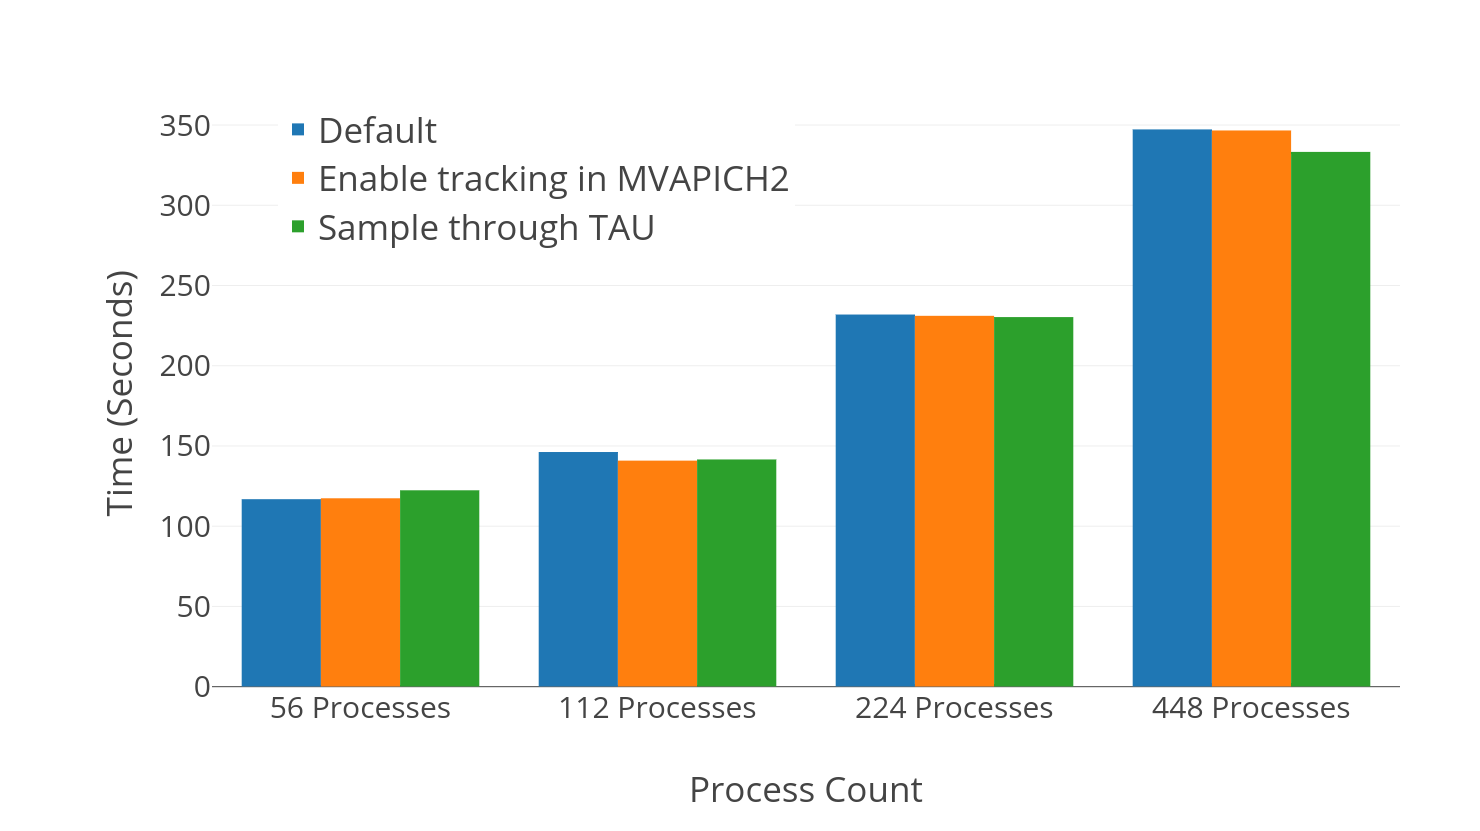
\includegraphics[width=\columnwidth,keepaspectratio,scale=1.0]{figures/MPI_T_Overheads}
                \captionsetup{justification=centering}
                  \caption{Overhead in enabling MPI\_T for 3DStencil}
                   \label{fig:overheads}
        \end{figure*}
\end{center}


\begin{center}
        \begin{figure*}[tbp!]
                 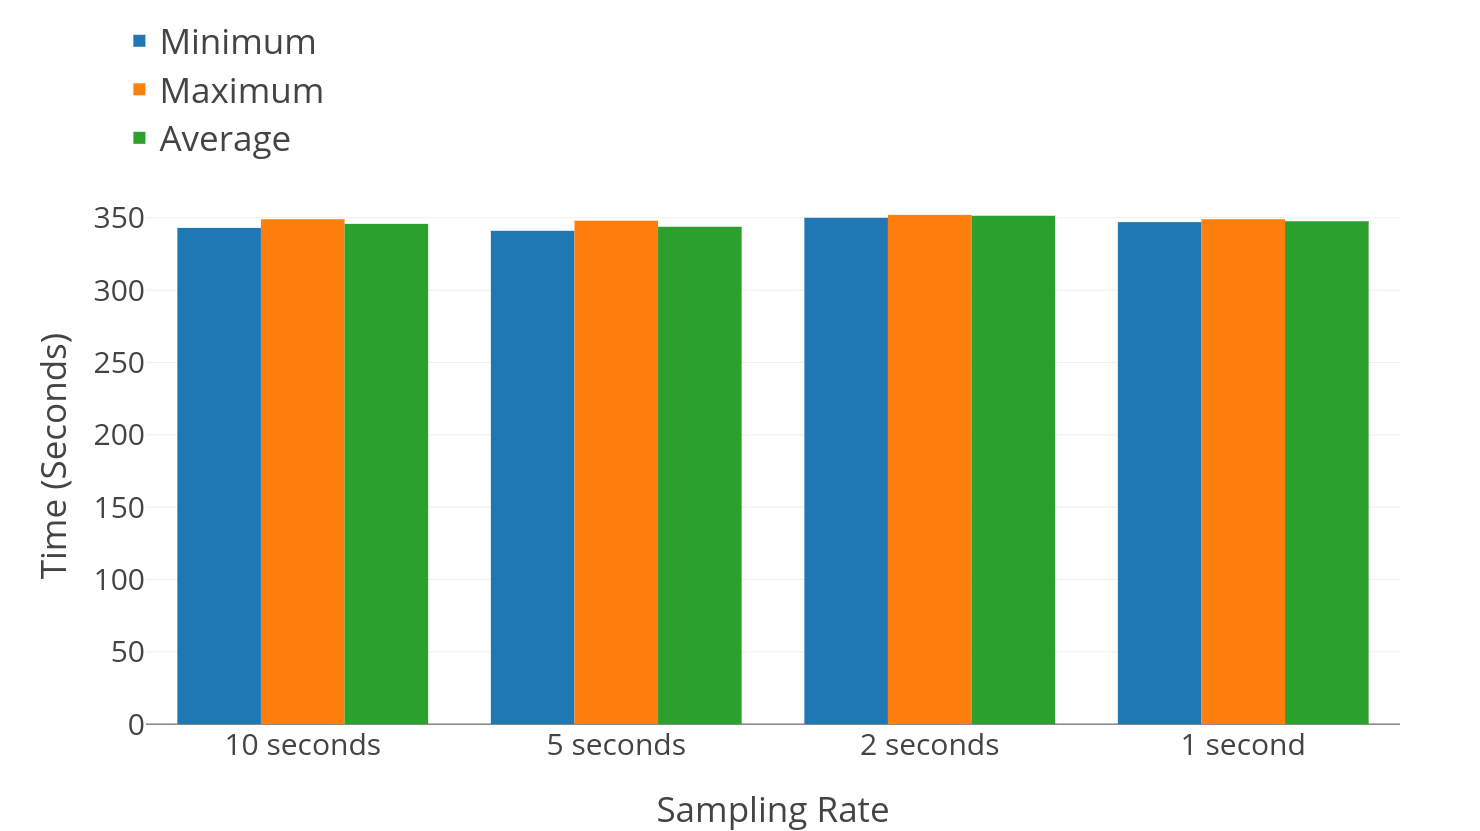
\includegraphics[width=\columnwidth,keepaspectratio,scale=1.0]{figures/MPI_T_Sampling_Frequently}
                \captionsetup{justification=centering}
                  \caption{Effect of MPI\_T sampling frequency on overhead for 3DStencil}
                   \label{fig:sampling_frequency}
        \end{figure*}
\end{center}

\section{Implementation Challenges and Issues}
\subsection{Deadlock Inside Signal Handler} 
The sampling mechanism inside TAU works by installing a signal handler to the \verb+SIGALRM+ signal. In order to prevent deadlocks, it is vital that all the callpaths inside the signal handler (TAU routines) are signal-safe, and only make signal-safe library calls. Our initial implementation of the autotuning plugin made free use of the \verb+malloc+ and \verb+calloc+ library calls --- these are not signal-safe. 
\par As it turned out, when running the TAU autotuning plugin with a large (300 or more) number of MPI processes, some processes were interrupted while inside a call to \verb+malloc+ from within the MVAPICH2 MPI library. As the plugin itself invoked \verb+malloc+, this led to a deadlock on the \verb+heap-lock+. This issue was mitigated by using TAU's custom memory manager to request for heap memory. A valuable lesson was learned in the process of detecting and resolving this issue --- a tool using interrupt-based sampling must make no assumption about the use of signal-unsafe routines inside the MPI library. In order to ensure proper functionality, tool writers' must always pessimistically assume that the library makes use of signal-unsafe routines, and design around this assumption.

\subsection {Supporting Dynamic Expansion of MPI\_T variables}
Recall that the number of PVARs and CVARs exported by the MPI library can increase (or decrease) at runtime. Supporting the case where the number decreases at runtime is trivial --- the tool just invalidates the PVARs (or CVARs) at the specific indices, and doesn't query the interface for variables at these indices.
\par Supporting the scenario where the number of variables \textit{increases} at runtime, however, is a more tricky task. As discussed earlier in this chapter, TAU maintains a \textit{user event} for every PVAR exported. In the default setup where TAU samples the MPI\_T interface inside a signal handler, TAU becomes aware of the increase in the number of variables only inside the signal handler. As a result, it needs to allocate the PVAR (CVAR) handles for the additional PVARs (CVARs), and create a TAU \textit{user event} for each of these additional PVARs (CVARs). Unfortunately, a call to the MPI\_T routine that allocates PVAR (CVAR) handles invokes a \verb+malloc+ call inside MVAPICH2. 
\par This leads to the same deadlock problem discussed previously. Moreover, at the time of detecting this issue, it was discovered that a lot of routines that lie in the callpath for the creation of a TAU \textit{user event} were signal-unsafe. As a result, it was decided that TAU would not support dynamic expansion of MPI\_T variables for the time being. 
\par The lesson here is --- sampling-based techniques for MPI\_T are bound to be limited by the use of signal-safe routines, and this tends to increase the complexity of the tool implementation. For instance, one workaround for TAU would have been to store the fact that the number of MPI\_T variables has increased (state information), and then invoke the handle allocation routines from within the PMPI wrapper for the next MPI call. In order for this solution to work perfectly, this check must be performed inside the PMPI wrapper for every MPI routine, thereby increasing the overall overheads for the TAU PMPI wrapper when MPI\_T is enabled. This solution was abandoned owing to the potential performance risks, and the manual work involved in implementing it.
\section{Summary}
This chapter has described the design and implementation of the MPI performance engineering architecture in TAU. We have also described the usage scenarios for this architecture and validated the design by performing experiments on synthetic and production scientific applications. The next chapter shall describe the MPI\_T based performance introspection support in Caliper. 
